\documentclass[10 pt,usenames,dvipsnames, oneside]{article}
\usepackage{../../../modelo-ensino-medio}



\begin{document}

\begin{center}
  \begin{minipage}[l]{3cm}

\includegraphics[width=2cm]{logo}    
\end{minipage}\hfill
\begin{minipage}[r]{.8\textwidth}
 {\Large \scshape Atividade: Contando quadrados}  
\end{minipage}
\end{center}
\vspace{.2cm}

\ifdefined\prof
%Habilidades da BNCC
\begin{objetivos}
\item \textbf{EM13MAT403} Comparar e analisar as representações, em plano cartesiano, das funções exponencial e logarítmica para identificar as características fundamentais (domínio, imagem, crescimento) de cada uma, com ou sem apoio de tecnologias digitais, estabelecendo relações entre elas.
\end{objetivos}

%Caixa do Para o Professor
\begin{goals}
%Objetivos específicos
\begin{enumerate}
\item Investigar um modelo discreto de decaimento exponencial;
\item Identificar gráficos de funções exponenciais decrescentes e relacionar ao fator de crescimento;
\item Reconhecer o modelo exponencial em dados experimentais.
\end{enumerate}

\tcblower

%Orientações e sugestões
\begin{itemize}
\item Esta atividade é uma adaptação do experimento \textit{Eliminando Quadrados} (\url {https://m3.ime.unicamp.br/recursos/1008}) que faz parte da coleção  Matemática Multimídia da UNICAMP (\url{https://m3.ime.unicamp.br}) que oferece diversos recursos educacionais de Matemática para o ensino médio.
\item No item \titem{d)} as perguntam visam estimular conjecturas do tipo os números são sempre positivos, sempre menores que um, eventualmente são iguais a 0 ou 1, mas isso ocorre apenas para quantidades pequenas de quadradinhos, ficam próximos de $0{,}5$, etc. Estimule que eles registrem as razões que os levaram a tais conjecturas.
\item Discuta sobre o que ocorreria caso o número de quadradinhos fosse bem maior; veja se há interesse na turma em desenvolver um projeto de programação que simule os lançamentos.
\end{itemize}
\end{goals}

\bigskip
\begin{center}
{\large \scshape Atividade}
\end{center}
\fi

Em uma caixa há $240$ quadradinhos de papel cartão dupla face, verde de um lado e marrom do outro. Eles são lançados sobre a mesa e os quadrados com lado marrom para cima são retirados, restando apenas $126$ quadradinhos (verdes).

\begin{figure}[H]
\centering
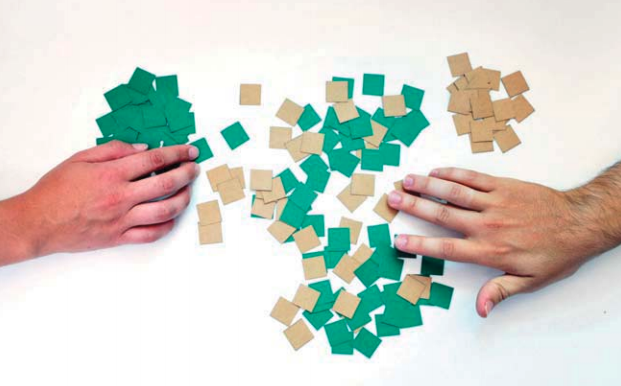
\includegraphics[width=250bp]{eliminando_quadrados.png}
\caption{Imagem retirada do experimento \textit{Eliminando Quadrados}, da coleção Recursos educacionais multimídia para a matemática do ensino médio. \url{https://m3.ime.unicamp.br/recursos/1008} }
\end{figure}


Um novo lançamento é feito e depois de retirados os marrons, sobram 68 verdes. Os lançamentos seguintes apresentam as seguintes quantidades de quadradinhos verdes:

\begin{center}
\begin{tabular}{|c|c|}
\hline
\tcolor{Lançamento} & \tcolor{\# verdes} \\ \hline
0 & $240$ \\ 
\hline
1 & $126$ \\ 
\hline
2 & $68$ \\ 
\hline
3 & $34$ \\ 
\hline
4 & $13$ \\ 
\hline
5 & $5$ \\ 
\hline
6 & $2$ \\ 
\hline
7 & $0$ \\ 
\hline
\end{tabular}
\end{center}

\begin{enumerate}

\item {}
Represente em um sistema de coordenadas os dados da tabela acima.

\item {}
Observando os dados da tabela é possível conjecturar que eles obedecem a algum padrão?

\item {} 
Acrescente uma terceira coluna à tabela contendo os quocientes entre as quantidades de um lançamento pela quantidade do lançamento anterior.

\begin{center}
\scalebox{.9}
{
\begin{tabular}{|c|c|c|}
\hline
\tcolor{Lançamento} & \tcolor{\# verdes} & \tcolor{quocientes} \\ 
\hline
0 & $240$ & --- \\ 
\hline
1 & $126$ & $\frac{126}{240}=0{,}525$\\ 
\hline
2 & $68$ & \\ 
\hline
3 & $34$ & \\ 
\hline
4 & $13$ &\\ 
\hline
5 & $5$ & \\ 
\hline
6 & $2$ & \\ 
\hline
7 & $0$ & \\ 
\hline
\end{tabular}
}
\end{center}

\item {}
Considerando outros resultados possíveis para o mesmo experimento, o que podemos esperar dos valores na terceira coluna da tabela? Que tipo de propriedades matemáticas esses números sempre terão? Que tipo de propriedade eles provavelmente terão?

\item {}
Um experimento como este descrito no item (a) pode ser simulado computacionalmente. Ao executar esta simulação 4 vezes, os seguintes resultados foram obtidos. 

$240, 113, 55, 28, 13, 7, 3, 0$ 

$240, 124, 66, 27, 16, 7, 3, 2, 2, 2, 0$ 

$240, 106, 57, 19, 9, 5, 1, 0$ 

$240, 124, 62, 29, 11, 5, 2, 1, 1, 0$

\item {}
Verifique se suas conjecturas se aplicam aos dados acima.

\item {}
Deduza uma expressão matemática que forneça, aproximadamente, a quantidade de quadradinhos verdes em função da ordem de lançamento.

\end{enumerate}


\ifdefined\prof
\begin{solucao}

	\begin{enumerate}
	\item {} 
	\adjustbox{valign=t}
	{
	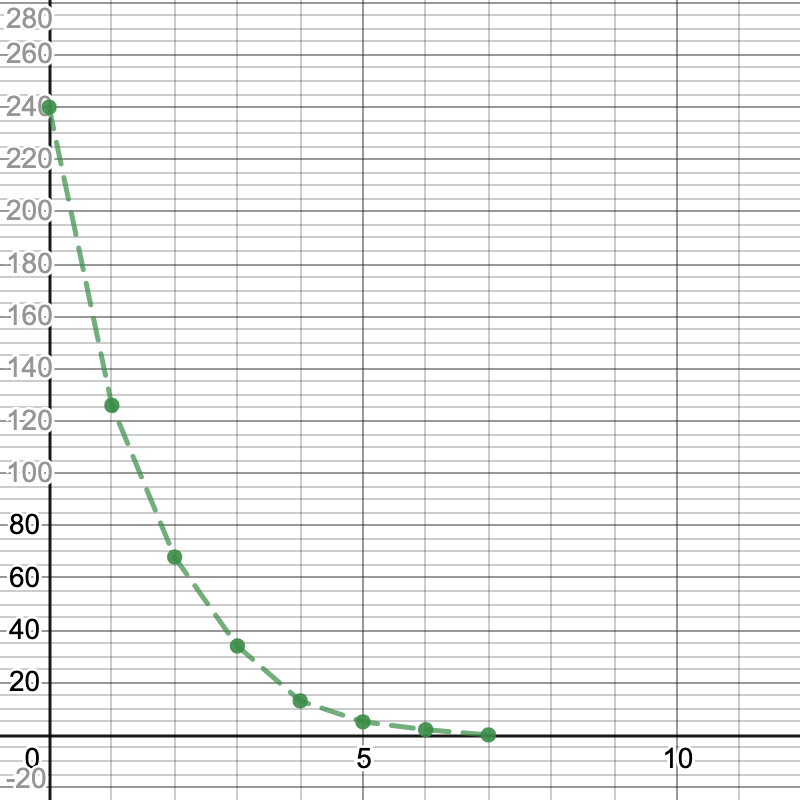
\includegraphics[width=.5\linewidth]{Contando_quadrados.png}
	}

	\item{}
	Observa-se que o número de quadrados com a face verde voltada para cima fica entre $40$ e $50\%$ do valor anterior a cada lançamento. O valor zero do final acontece por causa da quantidade pequena de quadrados.

	\item{}
	\adjustbox{valign=t}
	{
	\begin{tabu} to \textwidth{|c|c|c|}
	\hline
	\tcolor{Lançamento} & \tcolor{\# verdes} & \tcolor{quocientes} \\ 
	\hline
	0 & $240$ & --- \\ 
	\hline
	1 & $126$ & $\frac{126}{240}=0{,}525$\\ 
	\hline
	2 & $68$ & $\frac{68}{126}\approx0{,}539$ \\ 
	\hline
	3 & $34$ & $\frac{34}{68}=0{,}5$ \\ 
	\hline
	4 & $13$ & $\frac{13}{34}\approx 0{,}382$\\ 	
	\hline
	5 & $5$ & $\frac{5}{13}\approx 0{,}384$\\ 
	\hline
	6 & $2$ & $\frac{2}{5}=0{,}4$\\ 
	\hline
	7 & $0$ & $\frac{0}{2}=0$\\ 
	\hline
	\end{tabu}
	}

	\item{}
	Algumas respostas possíveis: serão sempre números positivos, sempre menores ou iguais a um, o quociente tende a ficar próximo a $0,5$.

	\item{}
	Responder em concordância com o que foi conjecturado no item anterior.

	\item{}
	Expressão da forma $F(n)=240\times a^{n}$, em que $a$ é qualquer valor próximo a $0,5$.

	\end{enumerate}

\end{solucao}
\fi

\end{document}